\documentclass[11pt,a4paper]{article}
\usepackage{fontspec}
\usepackage{setspace}
\usepackage{amsmath,amsfonts,amssymb,amsthm}
\usepackage[margin=1.1in]{geometry}
\usepackage{graphicx}
\usepackage{subfigure}
\usepackage{listings}
\usepackage{booktabs,dcolumn}                     
\usepackage{fancyhdr}
\usepackage{bbm}
\usepackage{multirow}
\usepackage{booktabs}
\usepackage{harvard}
\usepackage{enumerate}
\newcommand{\ra}[1]{\renewcommand{\arraystretch}{#1}}
\DeclareMathOperator{\tr}{tr}
\DeclareMathOperator{\vect}{vec}
\makeatletter
\newcommand*{\rom}[1]{\expandafter\@slowromancap\romannumeral #1@}
\makeatletter

\setstretch{1.4}
\setlength{\headheight}{15pt} 
\graphicspath{{graphs/}}  

\newtheorem{sectheorem}{Example}

 
\begin{document}
\title{Applied Survival Analysis - January 2016\\Solutions to Lab 7: Assessing the PH Assumption}
\date{\vspace{-10ex}}
\author{\vspace{-10ex}}
\maketitle
We first import the data in \verb|R|, and then have a look at the dataset.
\begin{spacing}{1.2}
\begin{footnotesize}
\begin{verbatim}
> ##########################################
> ### LAB 7: Assessing the PH Assumption ###
> ##########################################
> 
> # Import the data
> nurshome = read.csv("C:/Applied_Survival_Analysis_Jan2016/lab7/data/nurshome.csv")
> head(nurshome)
  los age rx gender married health fail
1 665  83  1      0       0      4    1
2 697  80  0      0       0      3    0
3   7  92  1      0       0      4    1
4 217  69  0      0       0      3    1
5 153  74  1      1       0      3    1
6  54  85  0      0       0      4    1
> 
> # Set the working directory
> setwd("C:/Applied_Survival_Analysis_Jan2016/lab7/graphs")
\end{verbatim}
\end{footnotesize}
\end{spacing}
\begin{enumerate}[(i)]
\item We have already seen that males have a shorter length of stay compared to females, and thus a higher hazard rate of discharge. Consequently, they have a higher cumulative hazard and therefore a higher log cumulative hazard. We expect this argument to be shown on the corresponding graphs.
\begin{spacing}{1.2}
\begin{footnotesize}
\begin{verbatim}
> # (i): Assessing the PH Assumption for gender and marital status separately
> # KM estimates by gender  (1=male, 0=female)
> library(survival)
> pdf("KMgender.pdf",height = 5.5,width = 5.5)
> fitKMgen = survfit( Surv(los,fail) ~ gender,data = nurshome)
> plot(fitKMgen,mark.time = F,fun = "cloglog",main = "Evaluation of PH Assumption",
+      xlab = "Length of Stay (days in log-scale)",lty = 1:2,col = c("blue","red"),
+      ylab = "Ln[-Ln(Survival Probabilities)]")
> legend("topleft",lty = 1:2,col = c("blue","red"),bty="n",legend = c("Female","Male"))
> dev.off()
\end{verbatim}
\end{footnotesize}
\end{spacing}
\newpage
Please, make sure you understand the way \verb|R| orders the survival curves on the graph below. Since \verb|gender=0| appears first and \verb|gender=1| follows
\begin{spacing}{1.2}
\begin{footnotesize}
\begin{verbatim}
> fitKMgen
Call: survfit(formula = Surv(los, fail) ~ gender, data = nurshome)

         records n.max n.start events median 0.95LCL 0.95UCL
gender=0    1173  1173    1173    902    144     123     164
gender=1     418   418     418    367     70      54      88
\end{verbatim}
\end{footnotesize}
\end{spacing}
we see that the first curve to be drawn is associated with females, whereas the second one corresponds to males (recall that 1=male and 0=female). Since there are two curves to be drawn, the options \verb|lty| (line type), \verb|col| (color of lines) and \verb|legend| (legend to be added to the graph) should all be vectors of size 2. Therefore, the first element in these options corresponds to females and the second element to males. Please, experiment with these rules to ensure that you have understood them.
\begin{figure}[htbp]
	\centering
		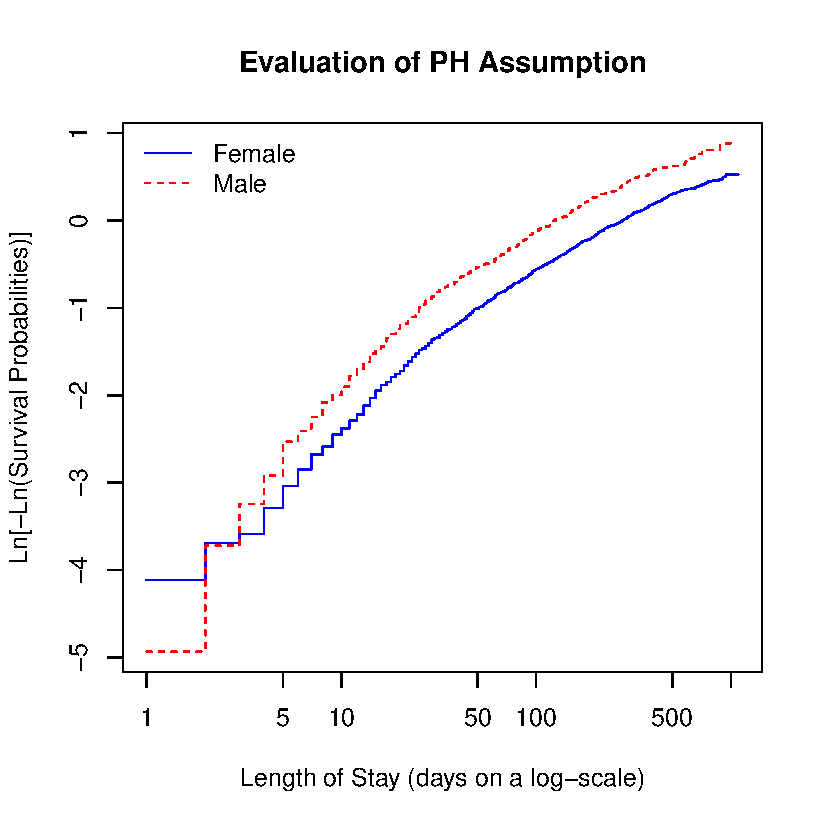
\includegraphics[scale=0.9]{KMgender.pdf}
		%\rule{35em}{0.5pt}
	\caption{Evaluation of PH assumption for gender.}
	\label{figure1}
\end{figure}

Don't pay too much attention to the curves for values up to 5 on the x-axis, as the curves are based on few data point in this range. Since the difference between the two curves is similar over time (they seem to be parallel), we have no reason to reject the assumption of proportional hazards.

We do the same for the effect of marital status
\begin{spacing}{1.2}
\begin{footnotesize}
\begin{verbatim}
> # KM estimates by marital status (1=married, 0=not married)
> fitKMmar = survfit( Surv(los,fail) ~ married,data = nurshome)
> 
> pdf("KMmarried.pdf",height = 5.5,width = 5.5)
> plot(fitKMmar,mark.time = F,fun = "cloglog",main = "Evaluation of PH Assumption",
+      xlab = "Length of Stay (days in log-scale)",lty = 1:2,col = c("blue","red"),
+      ylab = "Ln[-Ln(Survival Probabilities)]")
> legend("topleft",lty = 1:2,col = c("blue","red"),bty="n",
+        legend = c("Not married","Married"))
> dev.off()
\end{verbatim}
\end{footnotesize}
\end{spacing}

\begin{figure}[htbp]
	\centering
		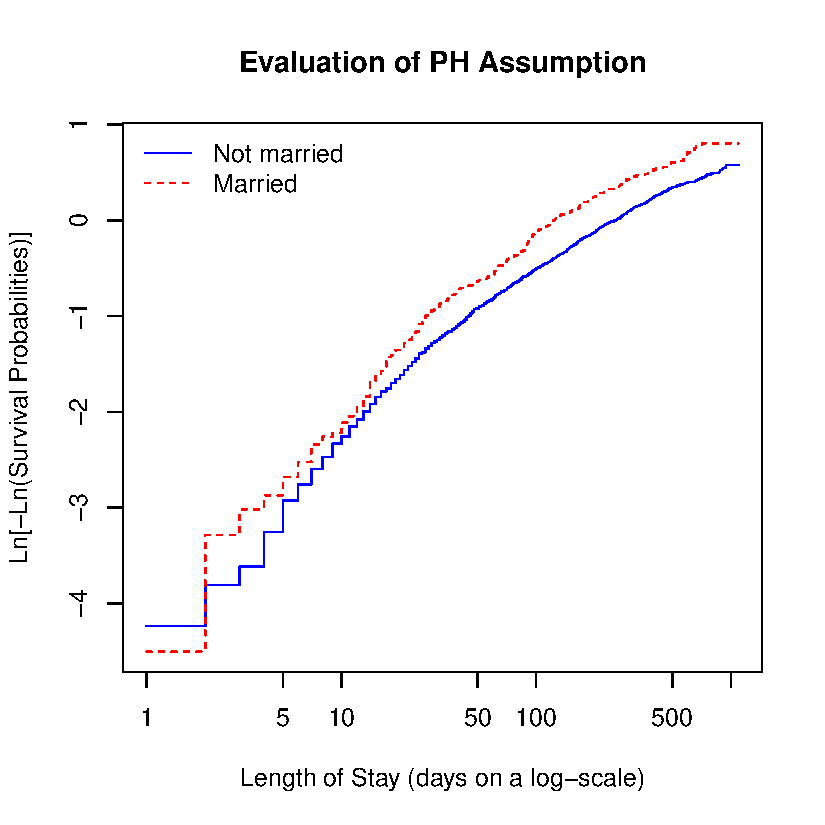
\includegraphics[scale=0.9]{KMmarried.pdf}
		%\rule{35em}{0.5pt}
	\caption{Evaluation of PH assumption for marital status.}
	\label{figure2}
\end{figure}

The  difference  between  the  two 
curves is similar over time, except for one point where the curves come near each other. As such, the PH assumption seems to be a reasonable assumption for the effect of marital status. 

Now, we'd like to compare the raw KM survival curves with those predicted by a Cox model. 
The closer the observed values are to the predicted ones, the less 
likely the proportional hazards assumption has been violated. 

To do this, we first have to fit a Cox PH model. Then, we use the \verb|survfit| function along with the \verb|newdata| option to specify the covariate values at which the predictions should be made. Finally, the \verb|plot| function can be used to produce a plot with the survival curves included in the \verb|survfit| object.
\begin{spacing}{1.2}
\begin{footnotesize}
\begin{verbatim}
> # Compare fitted with observed survival curves for gender
> fitCoxgen = survfit( coxph( Surv(los,fail) ~ gender,data = nurshome),
+                      newdata = data.frame(gender = c(0,1)) )
> 
> # First plot the fitted curves
> pdf("ExpVsObs_gen.pdf",height = 5.5,width = 5.5)
> plot(fitCoxgen,mark.time = F,xlab = "Length of Stay (days)",ylab = "Survival probability",
+      main = "Observed KM vs Predicted Survival Curves \nBy Categories of Gender",
+      lty = 1:2,col = c("blue","red"))
> # Add the raw curves
> lines(fitKMgen,lty = 3:4,col = c("green","orange"),mark.time = F)
> legend("topright",bty = "n",lty = 1:4,col = c("blue","red","green","orange"),
+        legend = c("Predicted: Female","Predicted: Male",
+                   "Observed: Female","Observed: Male"),ncol = 2,cex = 0.9)
> dev.off()
RStudioGD 
        2 
> 
> # Compare fitted with observed survival curves for married
> fitCoxmar = survfit( coxph( Surv(los,fail) ~ married,data = nurshome),
+                      newdata = data.frame(married = c(0,1)) )
> 
> # First plot the fitted curves
> pdf("ExpVsObs_mar.pdf",height = 5.5,width = 5.5)
> plot(fitCoxmar,mark.time = F,xlab = "Length of Stay (days)",ylab = "Survival probability",
+      main = "Observed KM vs Predicted Survival Curves \nBy Categories of Marital Status",
+      lty = 1:2,col = c("blue","red"))
> # Add the raw curves
> lines(fitKMmar,lty = 3:4,col = c("green","orange"),mark.time = F)
> legend("topright",bty = "n",lty = 1:4,col = c("blue","red","green","orange"),
+        legend = c("Predicted: Not married","Predicted: Married",
+                   "Observed: Not married","Observed: Married"),ncol = 2,cex = 0.9)
> dev.off() 
\end{verbatim}
\end{footnotesize}
\end{spacing}

\begin{figure}[htbp]
	\centering
		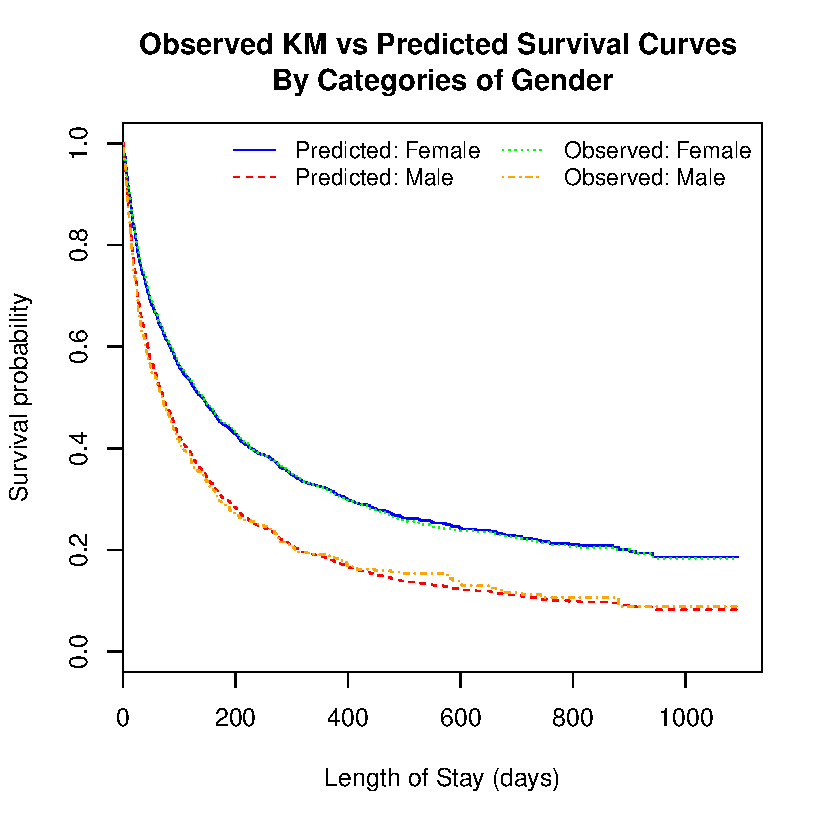
\includegraphics[scale=1]{ExpVsObs_gen.pdf}
		%\rule{35em}{0.5pt}
	\caption{Observed KM vs Predicted Survival Curves By Categories of Gender.}
	\label{figure3}
\end{figure}

\begin{figure}[htbp]
	\centering
		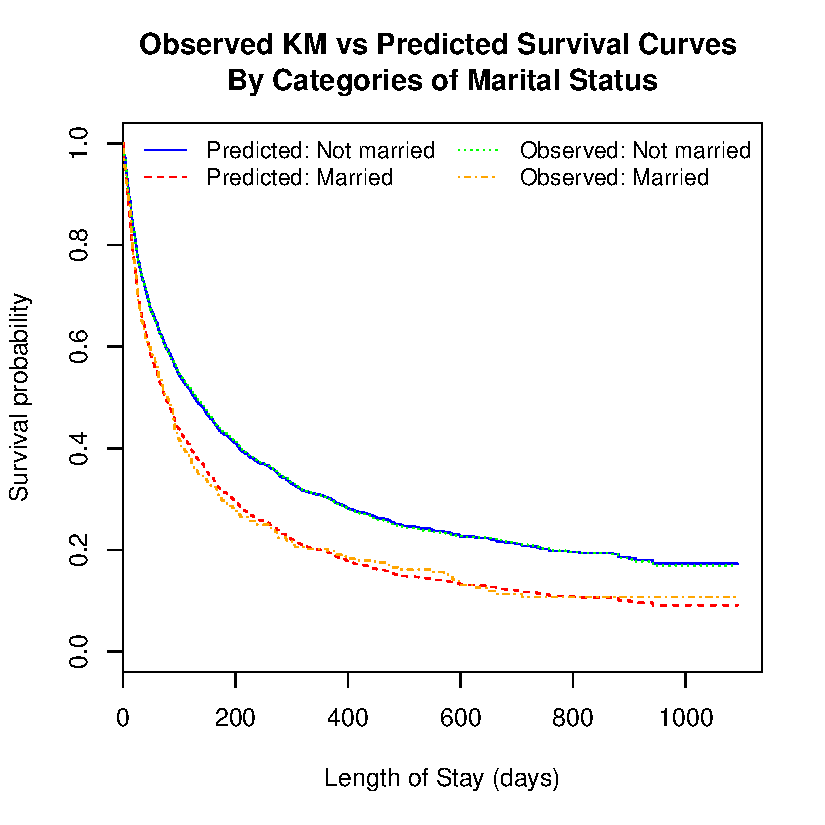
\includegraphics[scale=1]{ExpVsObs_mar.pdf}
		%\rule{35em}{0.5pt}
	\caption{Observed KM vs Predicted Survival Curves By Categories of Marital Status.}
	\label{figure4}
\end{figure}
Based on the graphs below, the observed and predicted survival probabilities seem to be pretty much in agreement. Therefore, there is no reason to doubt about the PH assumption for gender and marital status. 
\newpage
\item We generate a new variable that includes the combination of healthy and unhealthy men and women. Then, we create a new data frame that contains the groups of interest only.
\begin{spacing}{1.2}
\begin{footnotesize}
\begin{verbatim}
> # (ii): Generate a new variable
> nurshome$hlthsex = c( 1*(nurshome$gender==0 & nurshome$health==2) + 
+                       2*(nurshome$gender==1 & nurshome$health==2) +
+                       3*(nurshome$gender==0 & nurshome$health==5) +
+                       4*(nurshome$gender==1 & nurshome$health==5) )  
> table(nurshome$hlthsex)

   0    1    2    3    4 
1082  260   81  126   42 
> 
> # Create a new data.frame containing the groups of interest only
> nurshome2 = nurshome[nurshome$hlthsex!=0,]
> table(nurshome2$hlthsex)

  1   2   3   4 
260  81 126  42 
> 
> # Decode hlthsex as a factor variable
> nurshome2$hlthsex = factor(nurshome2$hlthsex,levels = 1:4,
+                            labels = c("Healthier Women","Healthier Men","Sicker Women" 
+                                       ,"Sicker Men"))
> # Fit KM curves
> fitKMgr = survfit( Surv(los,fail) ~ hlthsex,data = nurshome2)
> 
> # Let's have a look at the median survival times
> quantile(fitKMgr,probs = 0.5,conf.int = F)
                           50
hlthsex=Healthier Women 155.5
hlthsex=Healthier Men   100.0
hlthsex=Sicker Women     63.0
hlthsex=Sicker Men       30.0
> 
> pdf("KMhlthsex.pdf",height = 5.5,width = 5.5)
> plot(fitKMgr,mark.time = F,fun = "cloglog",ylab = "-Ln[-Ln(Survival Probabilities)]",
+      xlab = "Length of Stay (days in log-scale)",lty = 1:4,
+      col = c("blue","red","green","orange"),
+      main = "Evaluation of PH Assumption \nBy Categories of health-sex")
> legend("topleft",lty = 1:4,col = c("blue","red","green","orange"),bty = "n",
+        legend = c("Healthier Women","Healthier Men","Sicker Women","Sicker Men"))
> dev.off()
RStudioGD 
        2 
\end{verbatim}
\end{footnotesize}
\end{spacing}
\newpage
The differences between the above curves have a consistent sign during the majority of the follow-up. However, we can see that later in the study some groups cross. Thus, we may need a formal test to decide if the PH assumption holds.
\begin{figure}
	\centering
		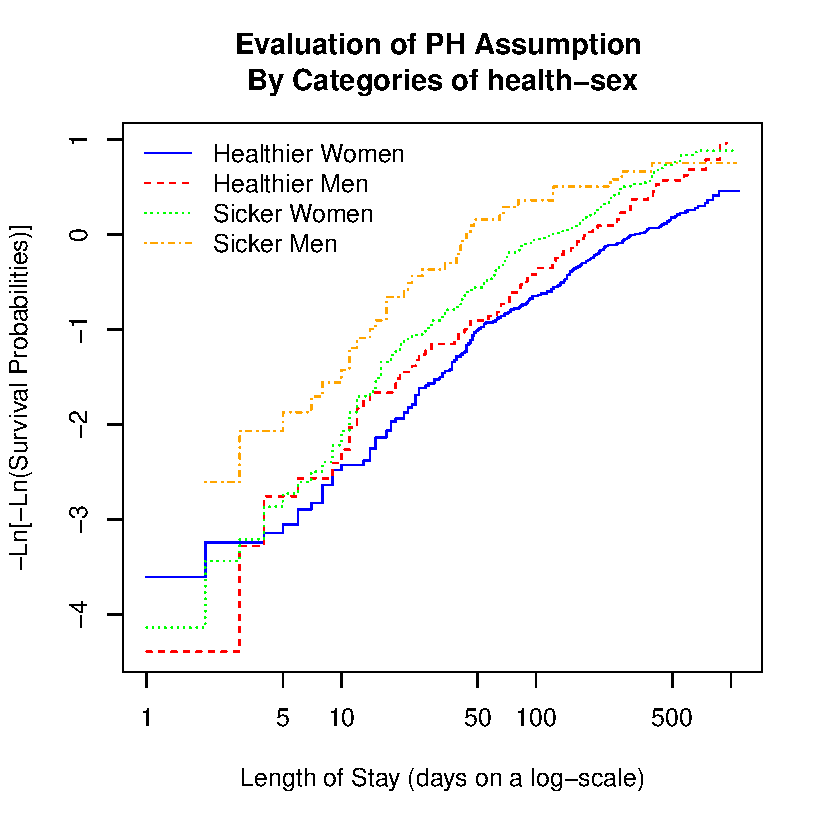
\includegraphics[scale=1]{KMhlthsex.pdf}
		%\rule{35em}{0.5pt}
	\caption{Evaluation of PH Assumption By Categories of health-sex.}
	\label{figure5}
\end{figure} 
\item We can fit a stratified Cox model by using the function \verb|strata|
\begin{spacing}{1.2}
\begin{footnotesize}
\begin{verbatim}
> # (iii): Cox model stratified by gender
> # We make the PH assumption for married and health, but NOT for gender
> fit = coxph( Surv(los,fail) ~ married + health + strata(gender),data = nurshome)
> summary(fit)
Call:
coxph(formula = Surv(los, fail) ~ married + health + strata(gender), 
    data = nurshome)

  n= 1591, number of events= 1269 

           coef exp(coef) se(coef)     z Pr(>|z|)    
married 0.16101   1.17470  0.07720 2.086    0.037 *  
health  0.16897   1.18408  0.03128 5.402  6.6e-08 ***
---
Signif. codes:  0 ‘***’ 0.001 ‘**’ 0.01 ‘*’ 0.05 ‘.’ 0.1 ‘ ’ 1

        exp(coef) exp(-coef) lower .95 upper .95
married     1.175     0.8513     1.010     1.367
health      1.184     0.8445     1.114     1.259

Concordance= 0.55  (se = 0.011 )
Rsquare= 0.021   (max possible= 1 )
Likelihood ratio test= 33.97  on 2 df,   p=4.199e-08
Wald test            = 34.22  on 2 df,   p=3.702e-08
Score (logrank) test = 34.33  on 2 df,   p=3.518e-08
\end{verbatim}
\end{footnotesize}
\end{spacing}
\begin{itemize}
\item \textbf{Gender:} We make no assumption on the effect of gender as it's the stratification variable. Its effect is allowed to vary continuously over time, but we don't estimate it (at this stage).
\item \textbf{Married:} We assume that the difference in the log hazard rate of discharge between married and unmarried is the same over time after adjusting for the health status and gender.
\item \textbf{Health status:} We assume that each unit increase in the health status is associated with a specific difference in the log hazard rate of discharge after adjusting for the marital status and gender.
\end{itemize}
Note that when you use a stratified cox model, the estimated effects are adjusted for any
variables contained in the stratification variable!

Now, based on the above fitted cox model we can estimate the baseline survival function for males and females separately. Thus, we're going to obtain estimates that are adjusted for the health and marital status without being subject to the proportional hazards assumption. Then if the log-log transformation of these estimates yields approximately parallel curves, the PH may hold for gender in the presence of health and marital status.
\begin{spacing}{1.2}
\begin{footnotesize}
\begin{verbatim}
> # Here we use the default, i.e., we obtain survival estimates for males and females 
> # evaluated at the mean values of married + health.
> # You can use any other values through the option newdata
> fitCoxgen2 = survfit(fit)
> 
> pdf("KMadjGender.pdf",height = 5.5,width = 5.5)
> plot(fitCoxgen2,mark.time = F,ylab = "-Ln[-Ln(Survival Probabilities)]",fun = "cloglog",
+      xlab = "Length of Stay (days in log-scale)",lty = 1:2,col = c("blue","red"),
+      main = "Evaluation of PH Assumption \nStratification by Gender")
> legend("topleft",lty = 1:2,col = c("blue","red"),bty = "n",
+        legend = c("Female","Male"))
> dev.off()
RStudioGD 
        2 
\end{verbatim}
\end{footnotesize}
\end{spacing}

\begin{figure}[htbp]
	\centering
		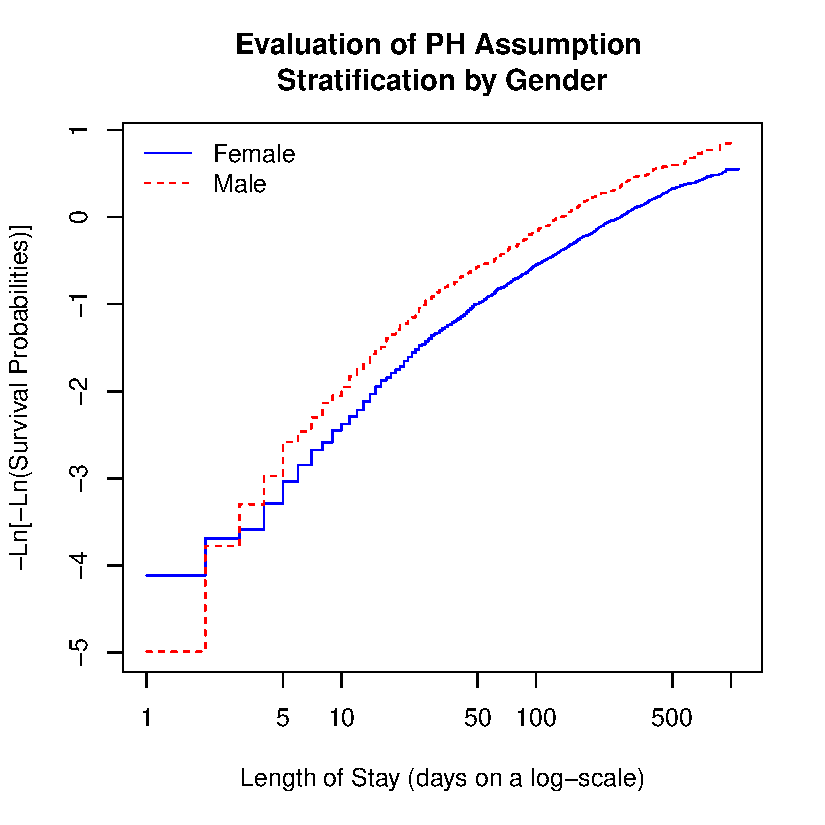
\includegraphics[scale=0.9]{KMadjGender.pdf}
		%\rule{35em}{0.5pt}
	\caption{Evaluation of PH assumption for gender after adjusting for marital and health status.}
	\label{figure6}
\end{figure}
There is 
no reason to reject the assumption of proportional hazards for gender even after adjusting for marital and health status. 
\end{enumerate}






















\end{document}